\chapter{Site Conditions and Design Inputs}
\section{Site Description and System Layout}

The Colebrooke Subdivision is located in the City of Florence, Rankin County, Mississippi, and consists of a planned residential development situated along the north side of Lewis Street. The site is characterized by gently rolling terrain and has been subdivided into residential lots connected by internal roadways and utility corridors as defined in the preliminary subdivision plat~\cite{ProjectD_Colebrooke_2020}. 

The sanitary sewer system within the subdivision is designed as a gravity collection network that conveys wastewater from individual residential lots toward a designated low point within the site. Due to the site’s topography, wastewater cannot be discharged directly to the municipal sewer system by gravity alone. As a result, a pump station is located at this low point to collect and lift the wastewater for conveyance to the downstream municipal connection.

The pump station serves as the transition point between the internal gravity sewer system and the external pressurized conveyance system. From the pump station, wastewater is transported through a short force main that connects to an existing municipal sewer manhole located along Lewis Street. The force main alignment follows the shortest practical route between the pump station and the downstream connection point to minimize pipe length and hydraulic losses.

The overall configuration of the system, including the subdivision layout, gravity sewer alignment, pump station location, and force main connection, is illustrated in Figure~\ref{fig:pump_layout}. The figure identifies the spatial relationship between system components and establishes the geometric framework that governs the hydraulic design presented in subsequent sections.

\begin{figure}[H]
\centering
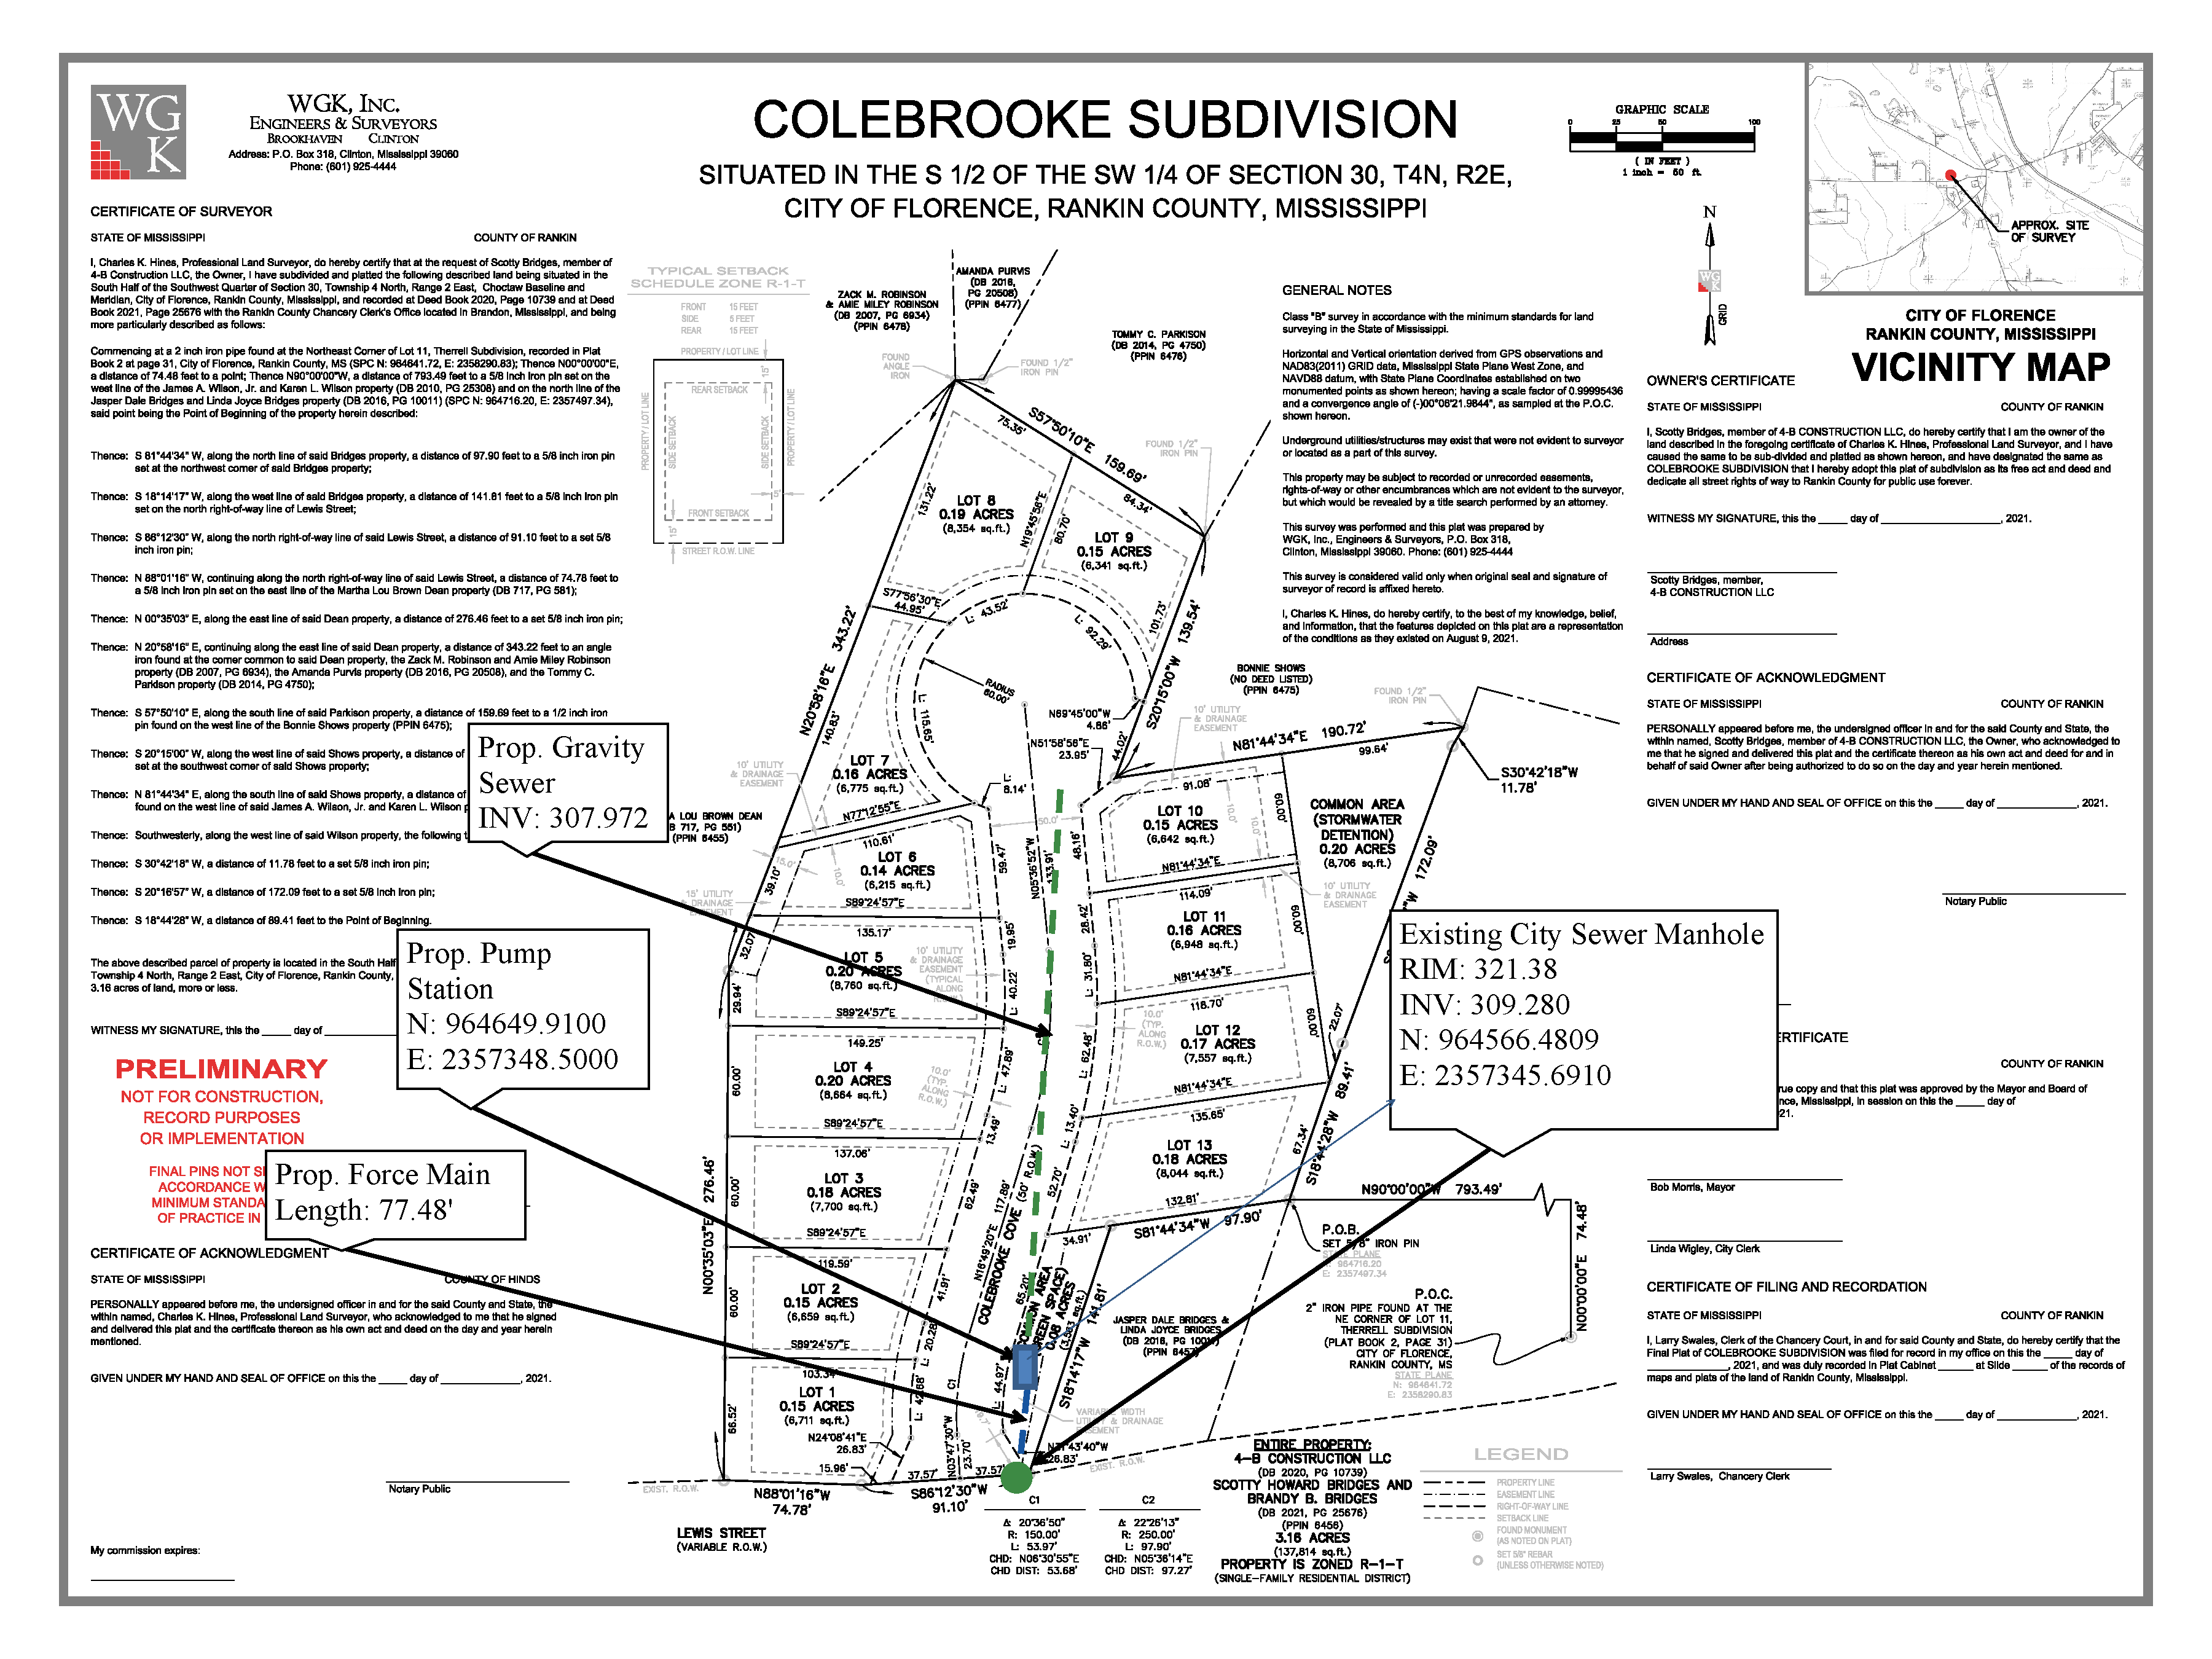
\includegraphics[width=\textwidth]{proposed_placement_plan_survey.pdf}
\caption{Proposed pump station location, gravity sewer alignment, and force main connection to existing municipal sewer manhole.}
\label{fig:pump_layout}
\end{figure}


\section{Wastewater Characteristics}

The conveyance system for the Colebrooke Subdivision is designed to transport domestic wastewater generated by residential units within the development. Unlike stormwater systems, which primarily convey runoff from precipitation events, sanitary sewer systems must handle wastewater containing suspended solids, organic matter, and other constituents typical of residential sewage.

The presence of suspended solids in wastewater introduces specific operational requirements for the conveyance system. In particular, the system must be capable of transporting solids without deposition, blockage, or excessive maintenance. This requirement influences both the hydraulic design of the force main and the selection of appropriate pumping equipment.

Wastewater lift stations are commonly equipped with submersible sewage pumps designed to operate under submerged conditions and convey both liquid and entrained solids. For residential wastewater applications, pumps are typically selected to accommodate the passage of solids of a specified size to ensure reliable operation. In this study, the system is assumed to handle solids up to approximately 3~inches in diameter, which is consistent with typical residential wastewater characteristics and standard pump capabilities.

These wastewater characteristics establish the functional requirements for the pump station and force main system, particularly with respect to maintaining adequate flow conditions and ensuring reliable transport of solids through the conveyance system.



\section{Design Flow and System Inputs}

The hydraulic capacity of the pump station is governed by the wastewater flow entering the system from the subdivision gravity sewer network. The estimation of wastewater generation and peak flow conditions was performed by the sewer system design team as part of the overall subdivision design. For the purpose of this analysis, the peak flow value obtained from that evaluation is adopted as the governing design input.

The peak wastewater flow used for the pump station design is given by

\[
Q_{\text{peak}} = 12.46 \ \text{gpm}
\]

This value represents the maximum anticipated inflow to the pump station under peak operating conditions and is used as the basis for sizing the force main and selecting the pumping system.

In addition to flow, several geometric and hydraulic parameters define the system configuration and are required for subsequent analysis. These parameters are summarized in Table~\ref{tab:design_inputs}.

\begin{table}[H]
\centering
\caption{Design Inputs}
\label{tab:design_inputs}
\begin{tabular}{llll}
\toprule
\textbf{Parameter} & \textbf{Value} & \textbf{Unit} & \textbf{Source} \\
\midrule
Peak wastewater flow & 12.46 & gpm & Sewer design team \\
Force main length & 77.48 & ft & Site plan and survey \\
Discharge invert elevation & 309.28 & ft & Site plan and survey \\
Wet well operating level & 299.00 & ft & Pump station layout \\
\bottomrule
\end{tabular}
\end{table}

The spatial configuration of the system is defined by the relative locations of the pump station and the downstream municipal sewer connection. The approximate coordinates of these points are provided below for reference.

\textbf{Proposed pump station location}

N 964649.9100 \\
E 2357348.5000

\textbf{Existing municipal sewer manhole location}

N 964566.4809 \\
E 2357345.6910

The pressure force main connects these two points and extends approximately 77.48~ft. The system layout, including the gravity sewer alignment, pump station location, and force main connection, is illustrated in Figure~\ref{fig:pump_layout}. This configuration establishes the geometric framework used in the hydraulic analysis presented in subsequent sections.


\section{Site Elevations and Hydraulic Constraints}

The hydraulic performance of the pump station system is primarily governed by the elevation difference between the wastewater level in the wet well and the downstream municipal sewer connection. This elevation difference defines the static head that must be overcome to convey wastewater from the subdivision to the existing sewer system.

For the Colebrooke Subdivision, the operating water level within the pump station wet well is approximately 299.00~ft, while the invert elevation of the downstream municipal sewer manhole is approximately 309.28~ft. The vertical difference between these elevations establishes the static elevation rise required for wastewater conveyance.

The static head is calculated as

\[
H_{\text{static}} = 309.28\ \text{ft} - 299.00\ \text{ft} = 10.28\ \text{ft}
\]

This value represents the minimum hydraulic head that must be provided by the pumping system to lift wastewater from the wet well to the discharge point. In addition to this elevation difference, the system must also overcome friction losses within the force main and minor losses associated with fittings, valves, and transitions.

The physical arrangement of the system, as illustrated in Figure~\ref{fig:pump_layout}, defines the hydraulic profile between the pump station and the municipal connection. The relatively short force main length and moderate elevation rise indicate that both static and frictional components will contribute to the total dynamic head required for system operation.

These elevation constraints establish the fundamental hydraulic requirements for the pump station and force main system. The total dynamic head, which incorporates both static and friction losses, will be evaluated in subsequent chapters to support the selection of an appropriate pump and conveyance configuration.


\section{Subsurface and Geotechnical Conditions}

A subsurface investigation was conducted for the Colebrooke Subdivision to evaluate soil and groundwater conditions relevant to the design and construction of infrastructure systems. The site is predominantly underlain by silty clay and clayey silt soils with varying degrees of stiffness and moisture content. Near-surface layers generally consist of softer, moisture-sensitive soils, while deeper layers exhibit increased stiffness.

Groundwater conditions across portions of the site are relatively shallow, which is consistent with the low-lying terrain and limited natural drainage. The combination of cohesive soils and elevated moisture content results in reduced shear strength and increased susceptibility to volume change, particularly under seasonal wetting and drying cycles.

These subsurface conditions influence several aspects of the pump station and force main design. Excavation for the wet well and pipeline installation requires consideration of soil stability and groundwater control to prevent collapse or excessive deformation. Proper trench bedding and backfill practices are necessary to ensure adequate support for the buried pipeline and to minimize settlement over time. In addition, the presence of groundwater necessitates attention to buoyancy effects and structural stability for the wet well.

Overall, the geotechnical conditions at the site require that construction and design approaches account for moisture-sensitive soils, groundwater influence, and long-term stability of underground infrastructure. These factors are incorporated into the design considerations presented in subsequent chapters.


\section{Existing Infrastructure Conditions}

The proposed wastewater conveyance system for the Colebrooke Subdivision is designed to discharge into an existing municipal sewer manhole located along Lewis Street. This manhole serves as the downstream connection point between the subdivision system and the City of Florence sanitary sewer network.

The internal gravity sewer system within the subdivision collects wastewater from residential lots and directs flow toward the proposed pump station. From this point, wastewater is conveyed through a short force main to the existing municipal manhole, where it enters the city’s gravity sewer system for further downstream transport and treatment.

The connection between the force main and the municipal manhole represents a critical interface in the overall system. This interface must ensure a smooth transition from pressurized flow within the force main to gravity flow within the municipal sewer system. Proper alignment and elevation compatibility between the discharge point and the existing sewer invert are necessary to maintain continuous flow and prevent backflow or hydraulic inefficiencies.

The layout of the proposed connection, including the relative positions of the pump station, force main, and municipal manhole, is illustrated in Figure~\ref{fig:pump_layout}. This configuration establishes the physical linkage between the subdivision infrastructure and the existing public sewer system.

The presence of an accessible municipal connection point allows the subdivision to integrate with the existing wastewater infrastructure without the need for extensive downstream modifications. As a result, the design focuses on ensuring compatibility between the proposed system and the existing network while maintaining reliable and efficient wastewater conveyance.
